\documentclass{idc_msc}

\title{Natural Language Processing \\\large Lecture 1}
\date{2019-03-05 \\ Last edited \currenttime\ \today}
\author{Lecture by Dr. Kfir Bar\\Typeset by Steven Karas}

\AtBeginDocument{\maketitle}
\AtEndDocument{\vfill\bibliographystyle{plain}\bibliography{../biblio}{}}

\usepackage{tikz-qtree}

\begin{document}

\paragraph{Disclaimer}

These notes are based on the lectures for the course Natural Language Processing, taught by Dr. Kfir Bar at IDC Herzliyah in the spring semester of 2018/2019.
Sections may be based on the lecture slides prepared by Dr. Kfir Bar.

\nocite{Jurafsky:2009:SLP:0131873210}
\nocite{manning1999foundations}
\nocite{DBLP:journals/corr/Goldberg15c}

% barkfir @ yahoo.com
% 054 4457771

\section{Course structure \& policy}

It is recommended to read the suggested papers before each class.


\section{Grading}

50\% homework assignments, 4 assignments.
50\% final project.

It will be allowed to work on projects together.
Homeworks will be submitted as a text file with a link to a Google Colab notebook.
We will use PyTorch, numpy, pandas, etc for homeworks.

A list of suggested projects will be published later in the course, and will also be done in pairs.

\section{Introduction}

Natural language processing is the study of having a computer understand human languages.
NLP is sometimes referred to as computational linguistics, but usually by linguists.
The three main facets of NLP are transformations:

\begin{enumerate}
  \item Unstructured text \(\to\) structured data
  \item Unstructured text \(\to\) unstructured text
  \item Structured data \(\to\) unstructured text
\end{enumerate}

A common application of NLP is chatbots, that answer simple queries in natural language.
The Turing Test is a famous test whereby a chatbot is indistinguishable from a human.
Eliza\cite{weizenbaum1966eliza} from 1966 was one of the first chatbots.
It used regular expressions to transform input statements into questions.

Historically, the field used rule based systems from the 50s until the 90s, at which point it became more data driven.
In the early aughts, machine learning took over, and since 2014 deep learning has taken over as the state of the art.
Deep learning generally treats the entire process as a black box to be trained, rather than using techniques such as bag of words, part of speech tags, etc.

NLP is a difficult field because sometimes the raw data is extremely dirty.
For example, garden path sentences, nonsense or spam input, idioms, ambiguous statements, etc.
Different dialects of a language also pose an issue, as do regional slang and turns of phrase.
For example, certain regions of British English are mutually intelligible yet wildly different from North American Vernacular English.

\subsection{Language}

There are approximately 7000 spoken languages in the world, but this number is obviously debated.
Languages are grouped into a hierarchy of families, usually based on their development and shared characteristics.

\paragraph{Zipf's Law}

The product of the frequency of words \(f\) and their rank \(r\) is approximately constant.

\subsection{NLP layers}

\begin{itemize}
  \item Phonetics - the sounds that words represent\footnote{Out of scope for this course}
  \item Morphology - word or word part structures
  \item Syntax - phrase structure; word modifiers
  \item Semantics - the literal meaning of words
  \item Pragmatics - conclusions of language
\end{itemize}

\section{Morphology}

\subsection{Segmentation/Tokenization}

A simple approach would be to simply split on whitespace.
A better approach would split on punctuation.

English is one of the easier languages to tokenize, but there are notable exceptions, for example "O'Hare" and "you've".
Many Asian languages have no spaces between words, and require more advanced approached.

\subsection{Morphology types}

\paragraph{Inflectional Morphology}

Words in different grammatical contexts can change the word.
For example, "duck" becomes "ducks" when it is plural.

\paragraph{Derivational Morphology}

Derivational morphology creates new words based on context for example "sense" becomes "nonsense".

\paragraph{Compounding}

Some languages such as German, Turkish, Inuktit, Finnish, etc combine base words into new words.

\subsubsection{Example: Hebrew}

Hebrew has 5000 roots, 50000 lemmas (dictionary entries), 2000000 prefix free words, 10000000 words, and about 10000000 speakers.
A single token can have up to 5 word parts: conjunction, article, preposition, stem, possession.

\subsection{Terminology}

\begin{description}
  \item[Token/Surface word] the complete word as written
  \item[Term] a unique token class
  \item[Morpheme] non recursive, sub word unit of a language
  \item[Stem] the word without prefixes or suffixes; the part that is common to all its inflected variants
  \item[Lemma] the canonical form of a word (the dictionary entry)
  \item[Root] in some languages, the primary lexical unit of a word
  \item[Affixes] a bound morpheme that modifies a word
\end{description}

\subsection{Part of Speech Tagging}

Given a sentence, we want to tag each word with the word types.
For example:

\begin{quote}
I want to book a flight to New York next week
\end{quote}

would become:

\begin{quote}
I /Pronoun, want /Verb, to /Preposition, book /Verb, a /Indefinite Article, flight /Noun, to /Preposition, New /Proper Noun, York /Proper Noun, next /Adjective, week /Noun
\end{quote}

\subsection{Sentence Segmentation}

A simple method would split on punctuation.
A more advanced approach is described in the suggested reading for next week, which considers a tagged corpus of sentence breaks.

\section{Syntax}

Forming grammatical phrases and sentences by putting words into structures.

\begin{center}
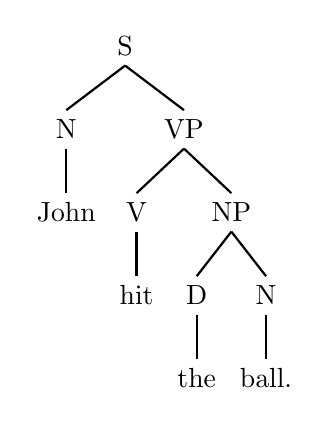
\begin{tikzpicture}
\tikzset{edge from parent/.append style={thick}}
\Tree [.S [.N John ]
          [.VP [.V hit ]
               [.NP [.D the ]
                    [.N ball. ]]]]
\end{tikzpicture}
\end{center}

\subsection{Ambiguous Syntax}

This is an example of a sentence where syntax helps resolve lexical ambiguities, as book can only be a verb in this sentence:

\begin{quote}
Did you book a ticket?
\end{quote}

This is a syntactically ambiguous sentence:

\begin{quote}
Bear left at zoo
\end{quote}

\subsection{Pathological Cases}

This is a syntactically valid English sentence:

\begin{quote}
Buffalo buffalo Buffalo buffalo buffalo buffalo Buffalo buffalo
\end{quote}

\begin{center}
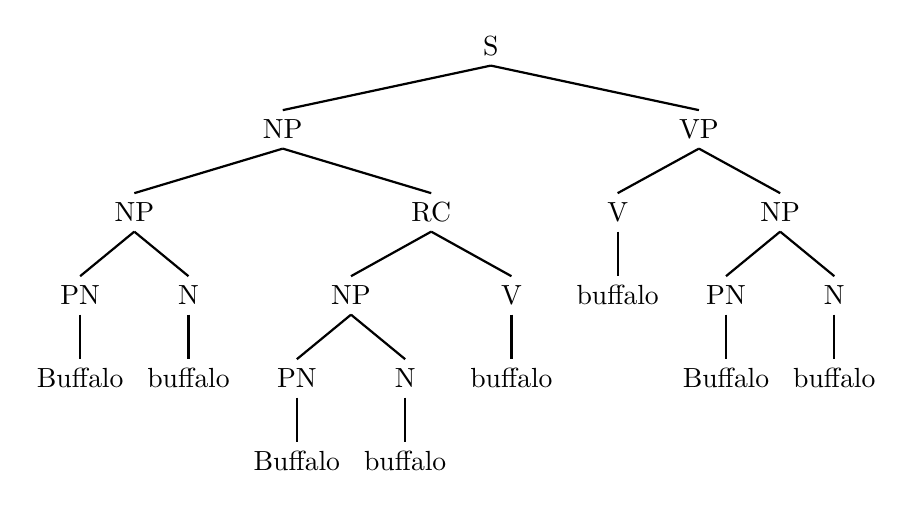
\begin{tikzpicture}
\tikzset{edge from parent/.append style={thick}}
\Tree [.S [.NP [.NP [.PN Buffalo ]
                    [.N buffalo ]]
               [.RC [.NP [.PN Buffalo ]
                         [.N buffalo ]]
                    [.V buffalo ]]]
          [.VP [.V buffalo ]
               [.NP [.PN Buffalo ]
                    [.N buffalo ]]]]
\end{tikzpicture}
\end{center}

\subsection{Sentence order}

I didn't have time to record this section. See slide 70.

\subsection{Dependency parsing}

See slide 72.

\end{document}
